\documentclass{article}
\usepackage{bera}
\usepackage{listings}
\usepackage{xcolor}
\usepackage{graphicx}
\usepackage{float}
\usepackage{hyperref}
\usepackage{tikz}
\usetikzlibrary{positioning,arrows.meta}


\colorlet{punct}{red!60!black}
\definecolor{background}{HTML}{EEEEEE}
\definecolor{delim}{RGB}{20,105,176}
\colorlet{numb}{magenta!60!black}

\lstdefinelanguage{json}{
    basicstyle=\normalfont\ttfamily,
    numbers=left,
    numberstyle=\scriptsize,
    stepnumber=1,
    numbersep=8pt,
    showstringspaces=false,
    breaklines=true,
    frame=lines,
    backgroundcolor=\color{background},
    literate=
     *{0}{{{\color{numb}0}}}{1}
      {1}{{{\color{numb}1}}}{1}
      {2}{{{\color{numb}2}}}{1}
      {3}{{{\color{numb}3}}}{1}
      {4}{{{\color{numb}4}}}{1}
      {5}{{{\color{numb}5}}}{1}
      {6}{{{\color{numb}6}}}{1}
      {7}{{{\color{numb}7}}}{1}
      {8}{{{\color{numb}8}}}{1}
      {9}{{{\color{numb}9}}}{1}
      {:}{{{\color{punct}{:}}}}{1}
      {,}{{{\color{punct}{,}}}}{1}
      {\{}{{{\color{delim}{\{}}}}{1}
      {\}}{{{\color{delim}{\}}}}}{1}
      {[}{{{\color{delim}{[}}}}{1}
      {]}{{{\color{delim}{]}}}}{1},
}

\lstdefinelanguage{log}{
    basicstyle=\small\ttfamily,
    numbers=left,
    numberstyle=\scriptsize,
    stepnumber=1,
    numbersep=8pt,
    showstringspaces=false,
    breaklines=true,
    frame=lines,
    backgroundcolor=\color{background},
    xleftmargin=1em,
    columns=fullflexible,
    morestring=[b]",
    comment=[l]{//},
    % Custom keyword and color definitions
    morekeywords={info,debug,error,warn,warning},
    keywordstyle=\color{blue!70!black}\bfseries,
    alsoletter={[,],:},
    literate=
      {[info]}{{\textcolor{blue}{[info]}}}1
      {[debug]}{{\textcolor{purple}{[debug]}}}1
      {[error]}{{\textcolor{red}{[error]}}}1
      {[warn]}{{\textcolor{orange!90!black}{[warn]}}}1
      {[warning]}{{\textcolor{orange!90!black}{[warning]}}}1
      {[Producer]}{{\textcolor{teal!70!black}{[Producer]}}}1
      {[Consumer]}{{\textcolor{olive!70!black}{[Consumer]}}}1
      {[Broker]}{{\textcolor{violet!70!black}{[Broker]}}}1
      {[Worker]}{{\textcolor{magenta!70!black}{[Worker]}}}1
      {[DigitalTwin]}{{\textcolor{cyan!70!black}{[DigitalTwin]}}}1
      {[NDN]}{{\textcolor{brown!70!black}{[NDN]}}}1
      {[HTTP]}{{\textcolor{gray!70!black}{[HTTP]}}}1
} 

\lstdefinelanguage{minindnconf}{
    basicstyle=\small\ttfamily,
    numbers=left,
    numberstyle=\scriptsize,
    stepnumber=1,
    numbersep=8pt,
    showstringspaces=false,
    breaklines=true,
    frame=lines,
    backgroundcolor=\color{background},
    xleftmargin=1em,
    columns=fullflexible,
    sensitive=true,
    % Comments (use # like many .conf files)
    morecomment=[l]{\#},
    commentstyle=\itshape\color{gray!70!black},
    % Treat these as part of words so highlighting works
    alsoletter={-:_[]},
    % Section headers / keys
    morekeywords={nodes,links,delay,nfd-log-level},
    keywordstyle=\bfseries\color{delim},
    % Common values
    morekeywords=[2]{DEBUG,INFO,WARN,ERROR,TRACE},
    keywordstyle=[2]\bfseries\color{purple!70!black},
    % (Optional) common node ids if you want them tinted
    morekeywords=[3]{a,b,c,d},
    keywordstyle=[3]\bfseries\color{teal!70!black},
    % Pretty-print punctuation and numbers/units
    literate=
      {=}{{\textcolor{punct}{=}}}{1}
      {:}{{\textcolor{punct}{:}}}{1}
      {[}{{\textcolor{delim}{[}}}{1}
      {]}{{\textcolor{delim}{]}}}{1}
      {_}{{\textcolor{gray!60!black}{\_}}}{1}
      {,}{{\textcolor{punct}{,}}}{1}
      % digits
      {0}{{{\color{numb}0}}}{1}
      {1}{{{\color{numb}1}}}{1}
      {2}{{{\color{numb}2}}}{1}
      {3}{{{\color{numb}3}}}{1}
      {4}{{{\color{numb}4}}}{1}
      {5}{{{\color{numb}5}}}{1}
      {6}{{{\color{numb}6}}}{1}
      {7}{{{\color{numb}7}}}{1}
      {8}{{{\color{numb}8}}}{1}
      {9}{{{\color{numb}9}}}{1}
      % units
      {ms}{{{\color{numb}ms}}}{2},
}


\begin{titlepage}
   \begin{center}
       \vspace*{1cm}
       
       \textbf{\LARGE Master Thesis - SeEDS (Secure and Efficient Data Namespace) }
       
       \vspace{1.5cm}
       \textbf{Author: Fotios Bistas, fot.bistas@aueb.gr}
       
       \textbf{Advisor: George Xylomenos, xgeorge@aueb.gr}
       
       \textbf{Reviewer: Vasilios Siris, vsiris@aueb.gr}
       
       \textbf{Reviewer: George Polyzos, polyzos@aueb.gr}

       \vspace{0.8cm}
            
       Department Name: Computer Science\\
       University Name: Athens University of Economics and Business\\
       Country: Greece\\
       Date: October 2025
       
       \vspace{0.8cm}

        
\includegraphics[width=0.9\textwidth]{images/opa.png}
   \end{center}
\end{titlepage}

\begin{document}

\section{Introduction}

A \textit{Data Space}, in the sense defined by ETSI ( European Telecommunications Standard Institute ), is a standards-based way
for many independent organizations to make their data discoverable and usable
to one another while each party keeps control of its own data. Instead of
moving everything into one central database, participants adopt common formats,
interfaces, and policies (identity, consent, usage rules) so they can share
data securely and auditably across organizational boundaries. This model aims
to break down today’s “data silos” ( isolated collections of data that prevent data sharing ) and enable new services that combine data
from multiple sources.

This differs from proprietary Content Delivery Networks (CDNs). CDNs focus on
fast distribution of static content (e.g., web assets, video) through
infrastructure operated by a single provider. In contrast, a Data Space
prioritizes interoperability, governance, and data sovereignty across many
owners, rather than speed of delivery from one centralized platform.

We have already implemented a simple Data Space based on the \textit{Named Data Networking (NDN)} architecture, in our previous project \textit{NGI Sargasso OC1 SNDS}. Named Data Networking (NDN) is a data-centric networking paradigm that shifts communication from host-based addressing (as in IP networks) to content-based addressing. In NDN, data are identified and retrieved directly by \textit{names} rather than by the location of the host that stores them. Each piece of data is cryptographically signed by its producer, ensuring authenticity and integrity regardless of where it is fetched from. This enables efficient in-network caching, data reuse, and intrinsic security properties that align naturally with the decentralized and self-sovereign principles of Data Spaces. Consequently, NDN networks are particularly well-suited for environments where multiple parties exchange data without relying on centralized servers or trusted intermediaries. Utilizing the NDN the system supported advanced data-driven applications over a fully distributed and self-sovereign identity framework.

Building upon SNDS, the \textit{Secure and Efficient Data Spaces (SeEDS)} project aims to deliver an ETSI-compliant Data Space solution. The project provides implementations for all required data API operations, including content filtering based on user-defined conditions, as well as optional temporal API operations that enable long-term data storage and retrieval. Specifically, this thesis implements the following goals regarding SeEDS:

\begin{itemize}
    \item Implement the full NGSI-LD API, including content filtering, temporal operations and event subscriptions.  
    \item Enhance data space efficiency by providing distributed data intermediaries and migrating content filters to their optimal location.
    \item Test the SeEDS implementation over the worldwide NDN testbed. 
\end{itemize}

The NGSI-LD API is a standardized interface for managing and exchanging
\emph{context information} in data spaces, as specified by ETSI. It provides a
common, HTTP-based framework that lets content providers, consumers, and
brokering services create, update, and query \emph{entities}, as well as
subscribe to change events. In NGSI-LD, each entity is represented in JSON-LD
and usually consists of a globally unique \texttt{id}, a \texttt{type} (its class),
and a set of \emph{attributes}. Attributes are either \emph{Properties} (values,
optionally with metadata such as \texttt{observedAt} or \texttt{unitCode}) or
\emph{Relationships} (links to other entities). A JSON-LD \texttt{@context}
binds the terms used to well-defined IRIs, ensuring semantic interoperability.

\begin{lstlisting}[language=json, caption={Example JSON-LD},label={lst:ngsi-ld-json}]
{ 
"@id": "urn:seeds:Car:001,
"@type": "Car,
"brand":{
    "type": "Property,
    "value": "BW
},
"dateVehicleFirstRegistered": { 
    "type": "Property
    "value": "201
    "emissionsCO2":{
        "type": "Property,
        "value": "2
    }
},
"@context":[
    "https://example.com/context.jsonl
] 
} 
\end{lstlisting}

This enables SeEDS to support two retrieval modes over its HTTP API: by \texttt{@id} and by \texttt{@type}.
A \emph{GET by ID} request retrieves a single JSON-LD entity given its globally
unique \texttt{@id}. A \emph{GET by TYPE} request retrieves all entities that
match the provided \texttt{@type}. Since \texttt{@type} is optional in SeEDS,
entities that omit it are treated as having the default \texttt{GENERIC} type.

\noindent\textbf{HTTP usage}
\begin{itemize}
  \item \textbf{GET by ID}: returns one entity
  \begin{verbatim}
  GET /?id=urn:seeds:car:car001
  \end{verbatim}

  \item \textbf{GET by TYPE}: returns an array of entities
  \begin{verbatim}
  GET /?type=Vehicle
  \end{verbatim}

  \item \textbf{Implicit type (default)}: entities without @type are treated as
  \texttt{GENERIC}
  \begin{verbatim}
  GET /?type=GENERIC
  \end{verbatim}
\end{itemize}

\noindent\textbf{Response shape}
\begin{itemize}
  \item GET by ID $\rightarrow$ a single JSON-LD object (the entity).
  \item GET by TYPE $\rightarrow$ a JSON array of JSON-LD entities.
\end{itemize}

\section{Architecture}

\subsection{SeEDS Service}

SeEDS bridges IP and NDN networks via two interfaces. First, it offers an
HTTP endpoint for exchanging NGSI-LD API messages with IP-based systems.
Second, it connects to the NDN Forwarding Daemon (NFD) through a netlink
socket to exchange NDN-specific messages with NDN nodes. Also each SeEDS Service contains a storage instance, where it stores data like locally published IDs, subscribed Nodes etc. The aforementioned are the components of the SeEDS Service. RV ( Rendezvous ) Nodes are nodes that can aggregate content and serve collections of it when queried to.

\begin{figure}[H]
    \centering
    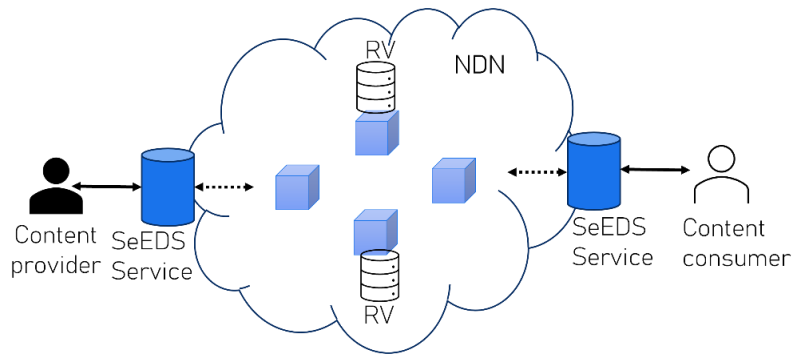
\includegraphics[width=0.8\linewidth]{images/seeds_architecture.png}
    \caption{High level SeEDS architecture.}
    \label{fig:seeds_architecture}
\end{figure}

\pagebreak

The following is the SeEDS Service components in detail: 

\begin{figure}[H]
    \centering
    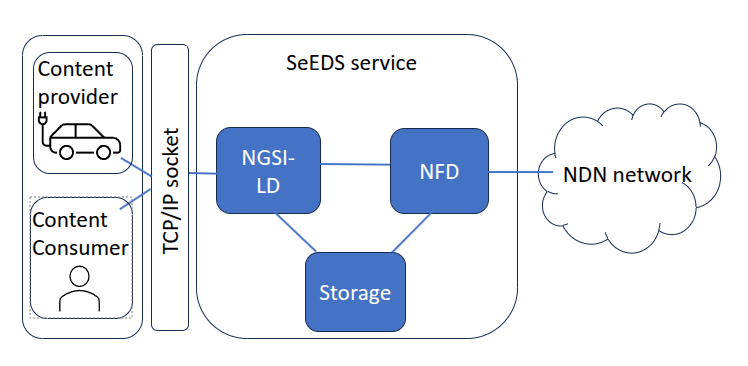
\includegraphics[width=0.8\linewidth]{images/seeds_service_detail.png}
    \caption{SeEDS Service in detail.}
    \label{fig:seeds_service_detail}
\end{figure}

The current architecture enables the SeEDS Service to perform the following operations: 

\begin{itemize}
    \item Consumers can create a \textit{HTTP GET} request to retrieve items from the NDN network. As mentioned before these are either \emph{GET by TYPE} or {GET by ID}. Note that the \textit{@type} and \textit{@id} need to be provided accordingly. 
    \item Providers can create \textit{HTTP POST} requests to provide/announce items to the NDN network. The service will also ensure that the data is stored inside its storage, ensuring that the data can be served when requested from some other node in the network. 
    \item Clients can also subscribe to a specific \textit{@id} or \textit{@type}. Since content in NDN is retrieved by its unique name rather than by host address, clients may express a request for a name even before the corresponding data is available. Once the data is published under that name, the network delivers it to all subscribed clients, enabling efficient and timely notifications.
    \item The NDN naming scheme also enables any NDN node to act as a \emph{Secondary} for another node within the network. A \emph{Secondary} node inherits the data of its corresponding \emph{Primary} node, including its storage contents, announced \textit{@ids}, \textit{@types} and \textit{subscriptions}. This design enhances the resilience of the SeEDS system, allowing it to recover the data of a failed node seamlessly and maintain service continuity.
\end{itemize}

\subsection{Resilience}

The resilience layer in SeEDS ensures that a \emph{Secondary} node continuously converges towards the state of a \emph{Primary} node through lightweight synchronization protocols built on NDN. At the core of this mechanism lies a versioned canonical JSON store on the \emph{Primary}, which exposes its state through a set of standardized NDN Interests and Data packets. The \emph{Secondary} maintains a local mirror of this store, applying updates received from the network and validating them against deterministic fingerprints.

The \emph{Primary} store maintains a bounded history of mutations. Each change increments a version counter, recomputes a canonical hash of the entire state, and records a snapshot to support future patch generation. It responds to queries with one of three data views: a lightweight metadata descriptor containing only the version and hash; a delta, represented as an RFC 6902 JSON Patch from one version to another; or a full snapshot of the canonical state. The \emph{Secondary} mirror accepts these responses and applies them locally. Whenever patch application fails, or when the requested patch is unavailable, the mirror falls back to a snapshot, ensuring eventual consistency even in the presence of divergence.

The resilience system is designed to handle failures gracefully. If the poller records consecutive failures in its liveness probes that exceed a configurable threshold, the \emph{Secondary} promotes itself to \emph{Primary} and terminates the polling loop. This self-promotion is communicated to the local services through IPC, ensuring that the system can continue to operate without interruption despite the failure of the original \emph{Primary}.

\begin{figure}[H]
    \centering
    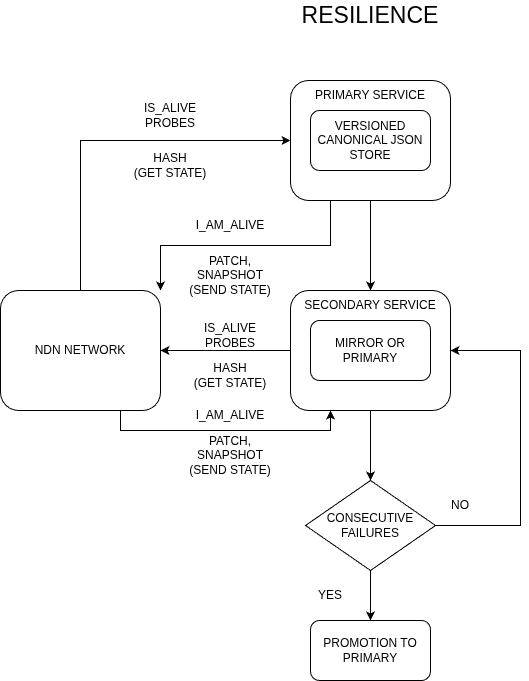
\includegraphics[width=0.8\linewidth]{images/resilience_seeds.png}
    \caption{Resilience architecture in SeEDS.}
    \label{fig:resilience_architecture}
\end{figure}

\section{Implementation}

The implementation described in this section reflects the state of the SeEDS system as of October 2025. As the project continues to evolve, certain design choices, component interfaces, or architectural details may change to accommodate new requirements, optimizations, or future redesigns. Therefore, this documentation should be considered a snapshot of the current implementation rather than a definitive or final version.


\subsection{Announcing Content}

When a node intends to announce content within the NDN network, it does so by advertising specific names. Consumers can then retrieve the corresponding content by \emph{expressing Interests} for these names. Each node in the network possesses a unique identifier (e.g., Node~1 on the left and Node~2 on the right). As illustrated in messages \emph{(0)} and \emph{(1)}, each node initially announces the base \textit{SeEDS} name concatenated with its unique identifier, forming the name \textit{SeEDS\textunderscore ID}. In addition, each node announces a \emph{scope} under a name of the form \textit{ID\textunderscore scopeID}. If a node is responsible for a particular registry or entity type—such as the \textit{CAR\textunderscore registry} in this example, shown in messages \emph{(2)} and \emph{(3)} —it also advertises the corresponding \textit{TYPE} and \textit{TYPE\textunderscore REGISTRY} names, enabling it to respond to Interests related to that registry.

\begin{figure}[H]
    \centering
    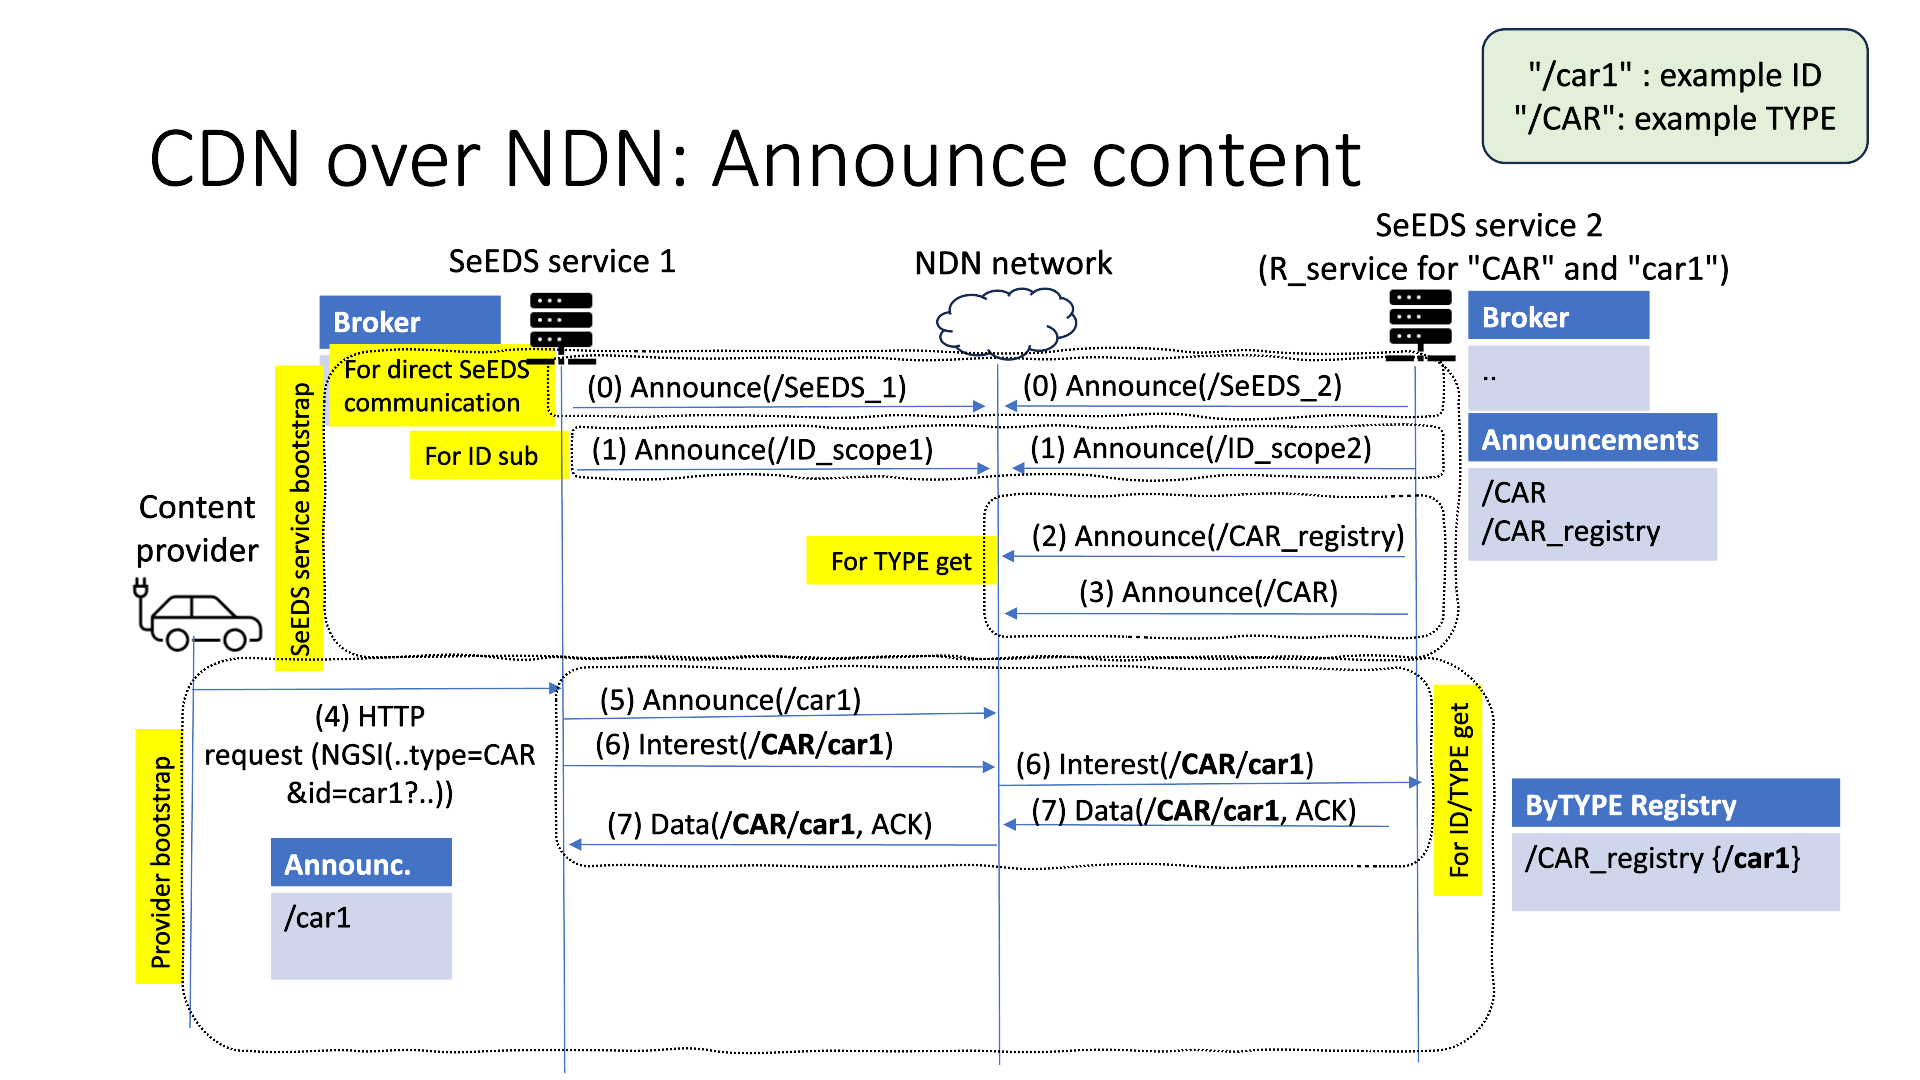
\includegraphics[width=0.8\linewidth]{images/announce_content.png}
    \caption{Announcing content inside the NDN network.}
    \label{fig:annoucing_content}
\end{figure}

Following the initial announcements, a new client intends to provide an entity with \textit{@id = car1} of type \textit{@type = CAR}. When this new \textit{@id} arrives, the receiving SeEDS Service first announces it locally, as illustrated in message~\emph{(5)}. It must then \emph{express an Interest}, as shown in message~\emph{(6)}, for the \textit{@type = CAR} registry so that the responsible node can store the new entry in the registry. The responsible node replies with an \emph{ACK} message, confirming that \textit{@id = car1} has been successfully registered under \textit{@type = CAR}. If the client’s \emph{HTTP request} does not explicitly specify a \textit{@type}, the system omits messages~\emph{(6)} and~\emph{(7)} and only announces the \textit{@id = car1} within the network.

\subsection{GET by ID}\label{get_by_id_section}



After an \textit{@id} is published into the network users can retrieve its content. Users create an \emph{HTTP Request} and specify the \textit{@id} that they want to retrieve, as shown in message \emph{(0)}. The SeEDS Service processes the message internally and \emph{expresses an interest} involving the \textit{@id=car1} inside the name, as shown in message \emph{(1)}. Note that messages~\emph{(0)} and~\emph{(1)} are identical in both the \emph{Direct} and \emph{Indirect} modes of the \texttt{GET by ID} operation. The choice of modes occurs dynamically depending on the data received by \textit{ProcessQueries()}. Moreover in both \emph{Direct} and \emph{Indirect} modes, the processing of filters occurs before the final data is returned to the user via the HTTP interface. Only the fields explicitly specified in the filter conditions are retained in the output. 


\subsubsection{Direct Mode}

\emph{Direct mode} occurs when the data processed by \textit{ProcessQueries()} is classified as a \emph{small payload}. In this case, the SeEDS Service responsible for the corresponding \textit{@id} responds \emph{directly} with the JSON payload, as illustrated in message~\emph{(2)}. The SeEDS Service that initially received the \emph{HTTP request} then forwards this data back to the client as the final response.

\begin{figure}[H]
    \centering
    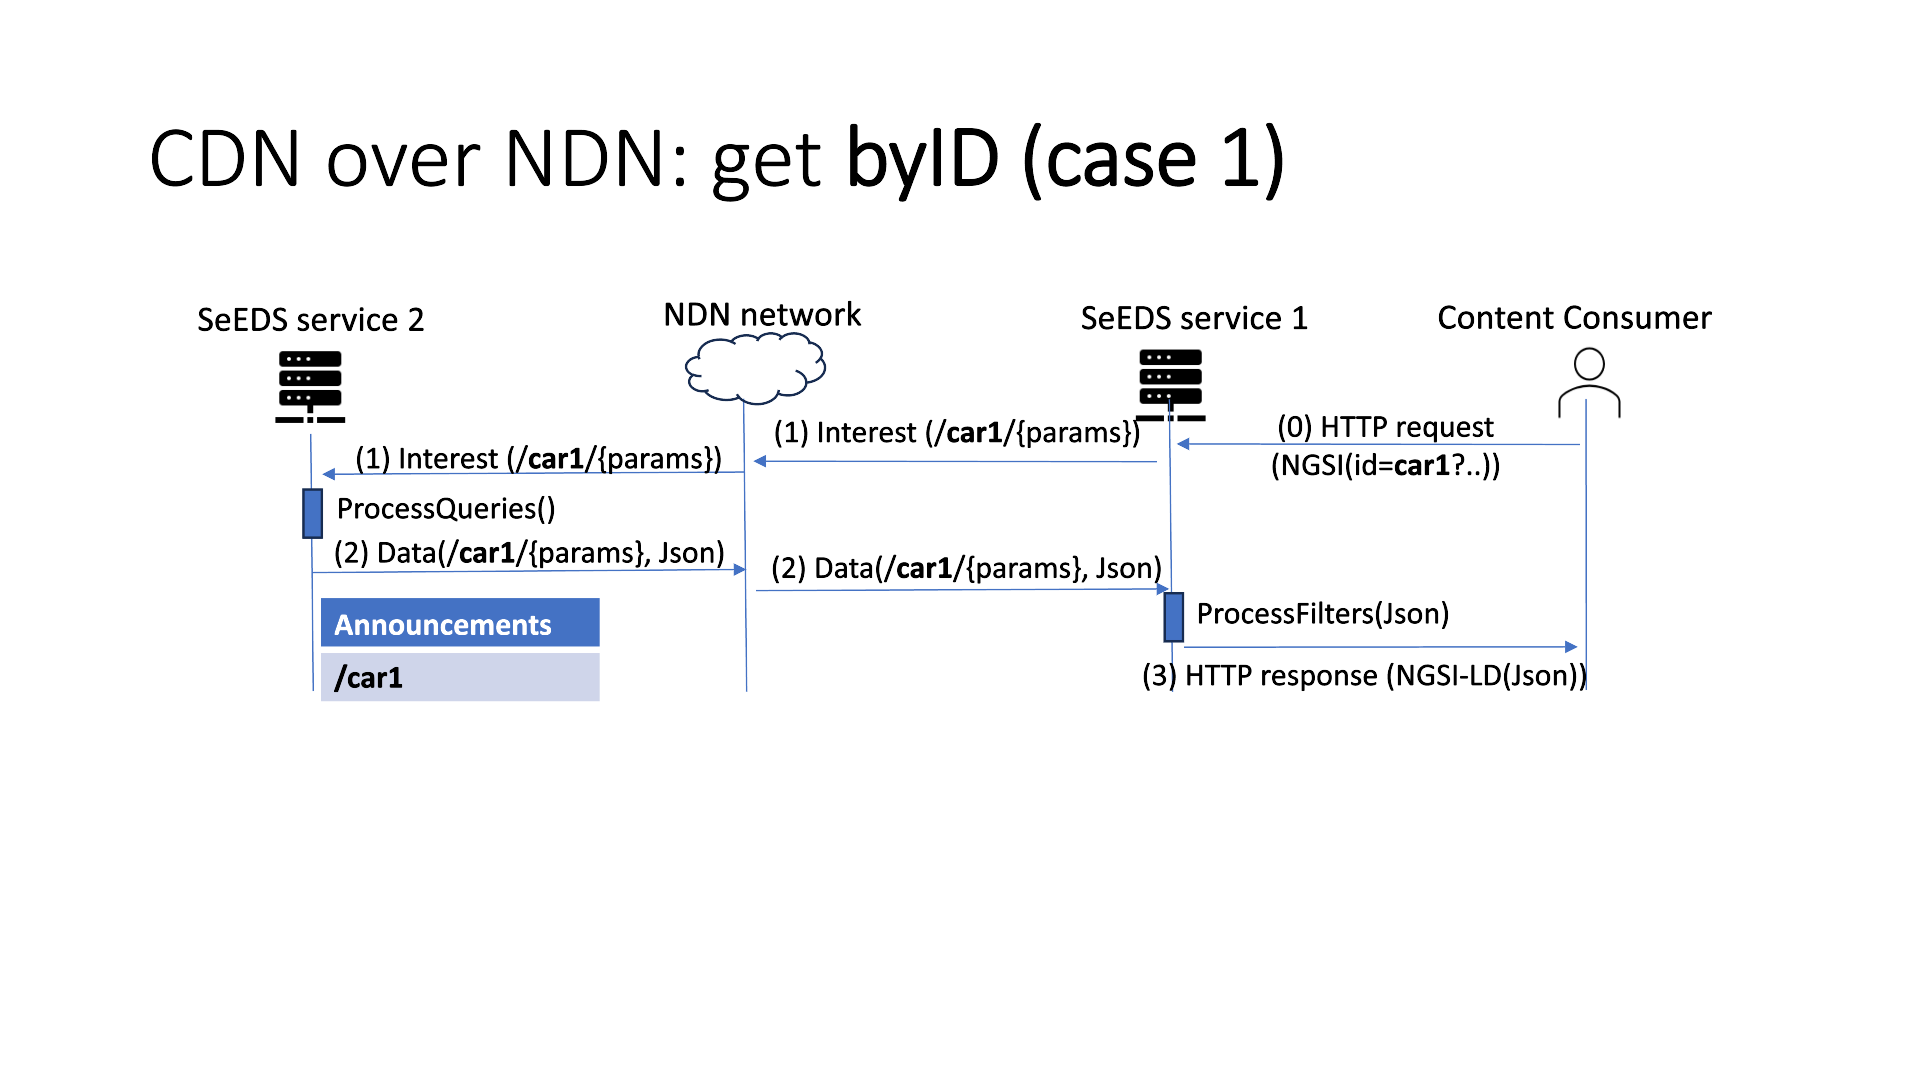
\includegraphics[width=0.8\linewidth]{images/get_by_id_direct.png}
    \caption{GET by ID direct mode.}
    \label{fig:get_by_id_direct}
\end{figure}

\subsubsection{Indirect Mode}

\emph{Indirect mode} occurs when the data processed by \textit{ProcessQueries()} is classified as a \emph{large payload}. In this case, the SeEDS Service responsible for the corresponding \textit{@id} does not transmit the full JSON directly. Instead, it responds with a \emph{metafile}, as illustrated in message~\emph{(2)}. The \emph{metafile} contains a list of \textit{@v\_ids}, which represent the individual \textit{@ids} along with their respective versions. Upon receiving the \emph{metafile}, the SeEDS Service that originally handled the \emph{HTTP request} proceeds to \emph{express Interests} for the specific \textit{@id} and each associated version. This effectively reinitiates the retrieval process in the same manner as a \emph{Direct mode} request, just for a specific version. The version can be represented in various forms, such as a timestamp, a numerical identifier, or any other scheme that uniquely distinguishes different instances of the same entity.


\begin{figure}[H]
    \centering
    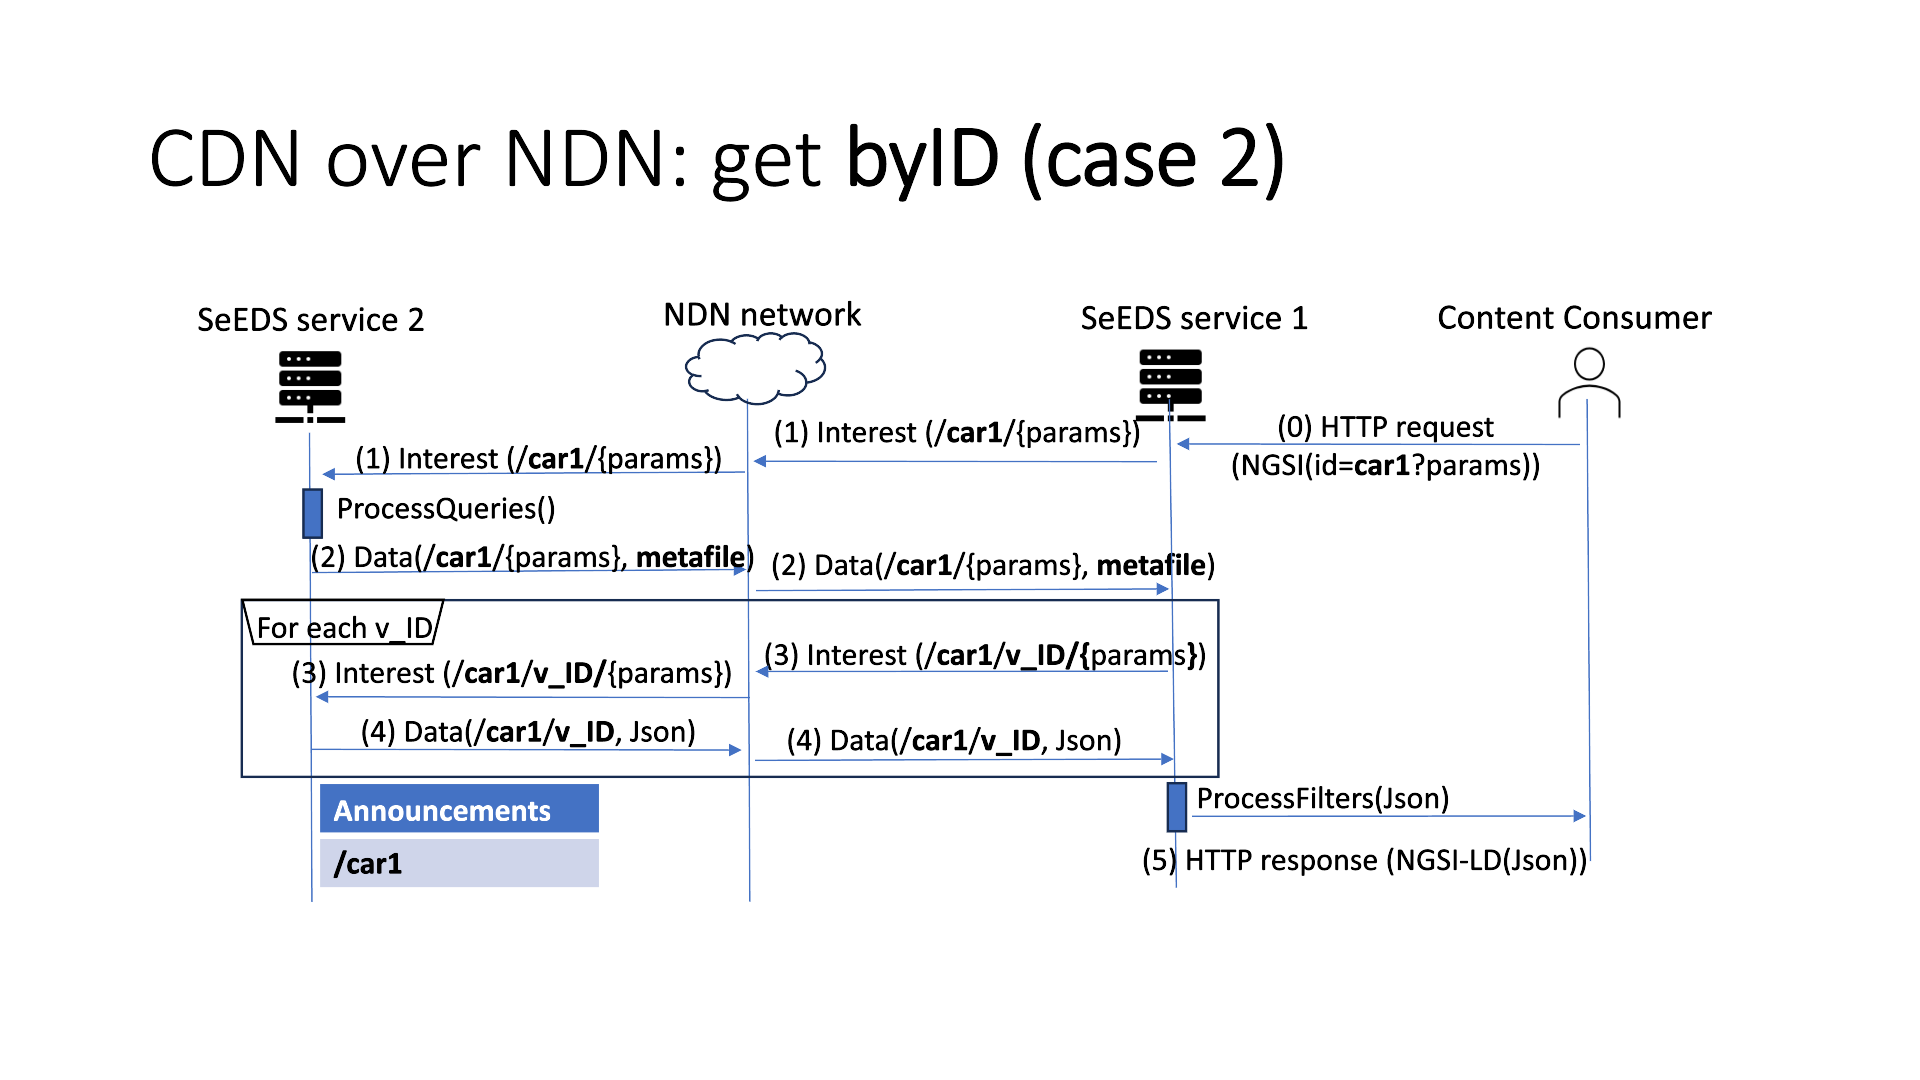
\includegraphics[width=0.8\linewidth]{images/get_by_id_indirect.png}
    \caption{GET by ID indirect mode.}
    \label{fig:get_by_id_indirect}
\end{figure}

\pagebreak 

\subsection{GET by TYPE}\label{get_by_type_section}

Users can also request data associated with a specific \textit{@type}. As illustrated in message~\emph{(0)}, the \emph{content consumer} specifies the desired \textit{@type} in the request sent to the SeEDS Service. The SeEDS Service that receives the \emph{HTTP Request} proceeds to \emph{express an Interest} in the NDN network, as shown in message~\emph{(1)}. The SeEDS Service responsible for the corresponding registry then receives this Interest and responds with the list of \textit{@ids} registered under that \textit{@type}, as shown in message~\emph{(2)}. After obtaining the list of \textit{@ids}, the SeEDS Service that originally handled the \emph{HTTP request} performs a separate \hyperref[get_by_id_section]{GET by ID} operation for each \textit{@id} to retrieve the associated data.

\begin{figure}[H]
    \centering
    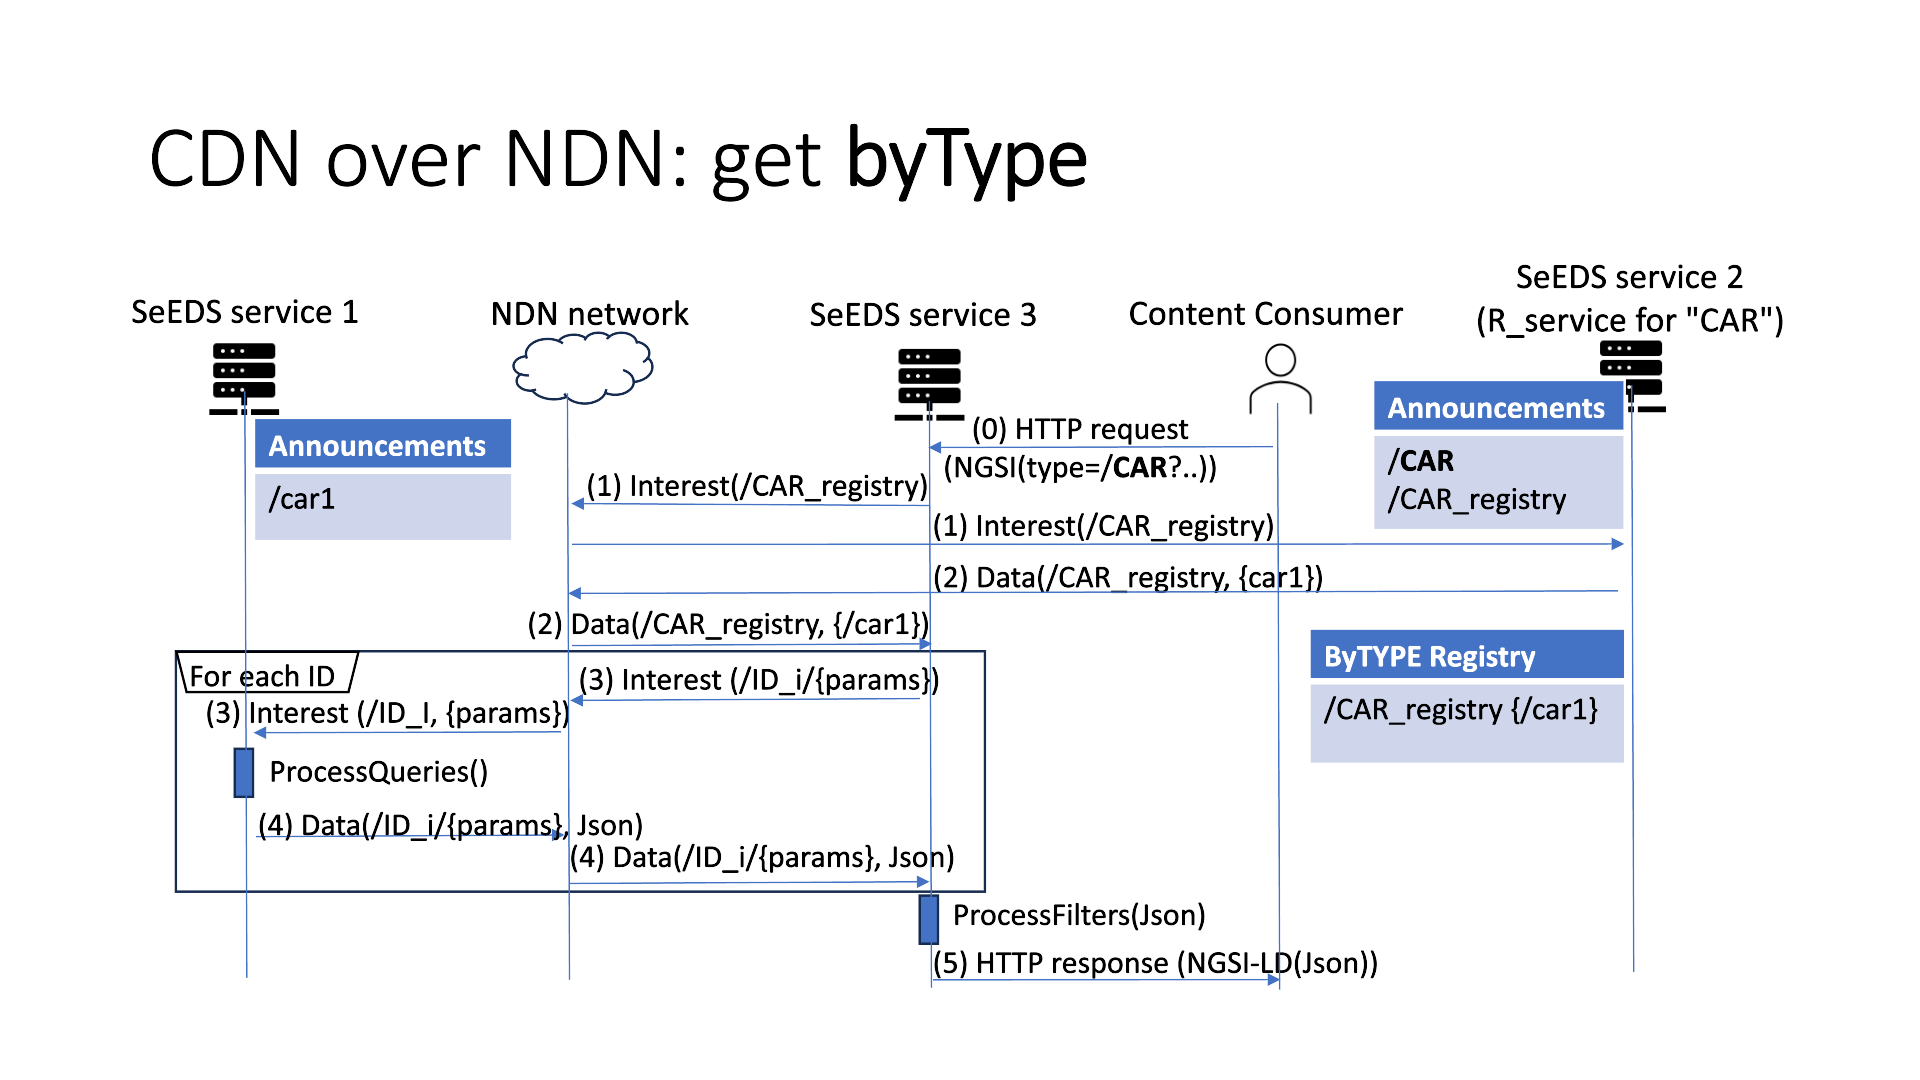
\includegraphics[width=0.8\linewidth]{images/get_by_type.png}
    \caption{GET by TYPE.}
    \label{fig:get_by_type}
\end{figure}

\pagebreak

\subsection{SUBSCRIPTIONS by ID}\label{subscriptions_by_id_section}

Consumers can also subscribe to a specific \textit{@id}. Once content associated with that \textit{@id} becomes available, the system automatically notifies the subscribed consumers and delivers the corresponding data. This mechanism allows consumers to subscribe to \textit{@ids} even before the data has been published. 

A consumer that wishes to subscribe to an \textit{@id} must specify the target identifier, as illustrated in message~\emph{(0)}. Upon receiving the \emph{HTTP request}, the SeEDS Service proceeds to \emph{express an Interest} containing both the responsible \emph{ID\_SCOPEID} for the given \textit{@id}—determined via a hashing function—and its own \emph{ID\_SCOPEID}, as shown in message~\emph{(1)}. When the responsible \emph{ID\_SCOPEID} receives this Interest, it records the sender’s \emph{ID\_SCOPE} as a subscriber for the specified \textit{@id} and responds with an \emph{ACK}, as depicted in message~\emph{(2)}.

When new data for the subscribed \textit{@id} is announced, the system checks for any existing subscribers and notifies them through their respective scopes that new content has become available, as shown in message~\emph{(3)}. The notified SeEDS Service then initiates a \hyperref[get_by_id_section]{GET by ID} operation to retrieve the newly published data.

\begin{figure}[H]
    \centering
    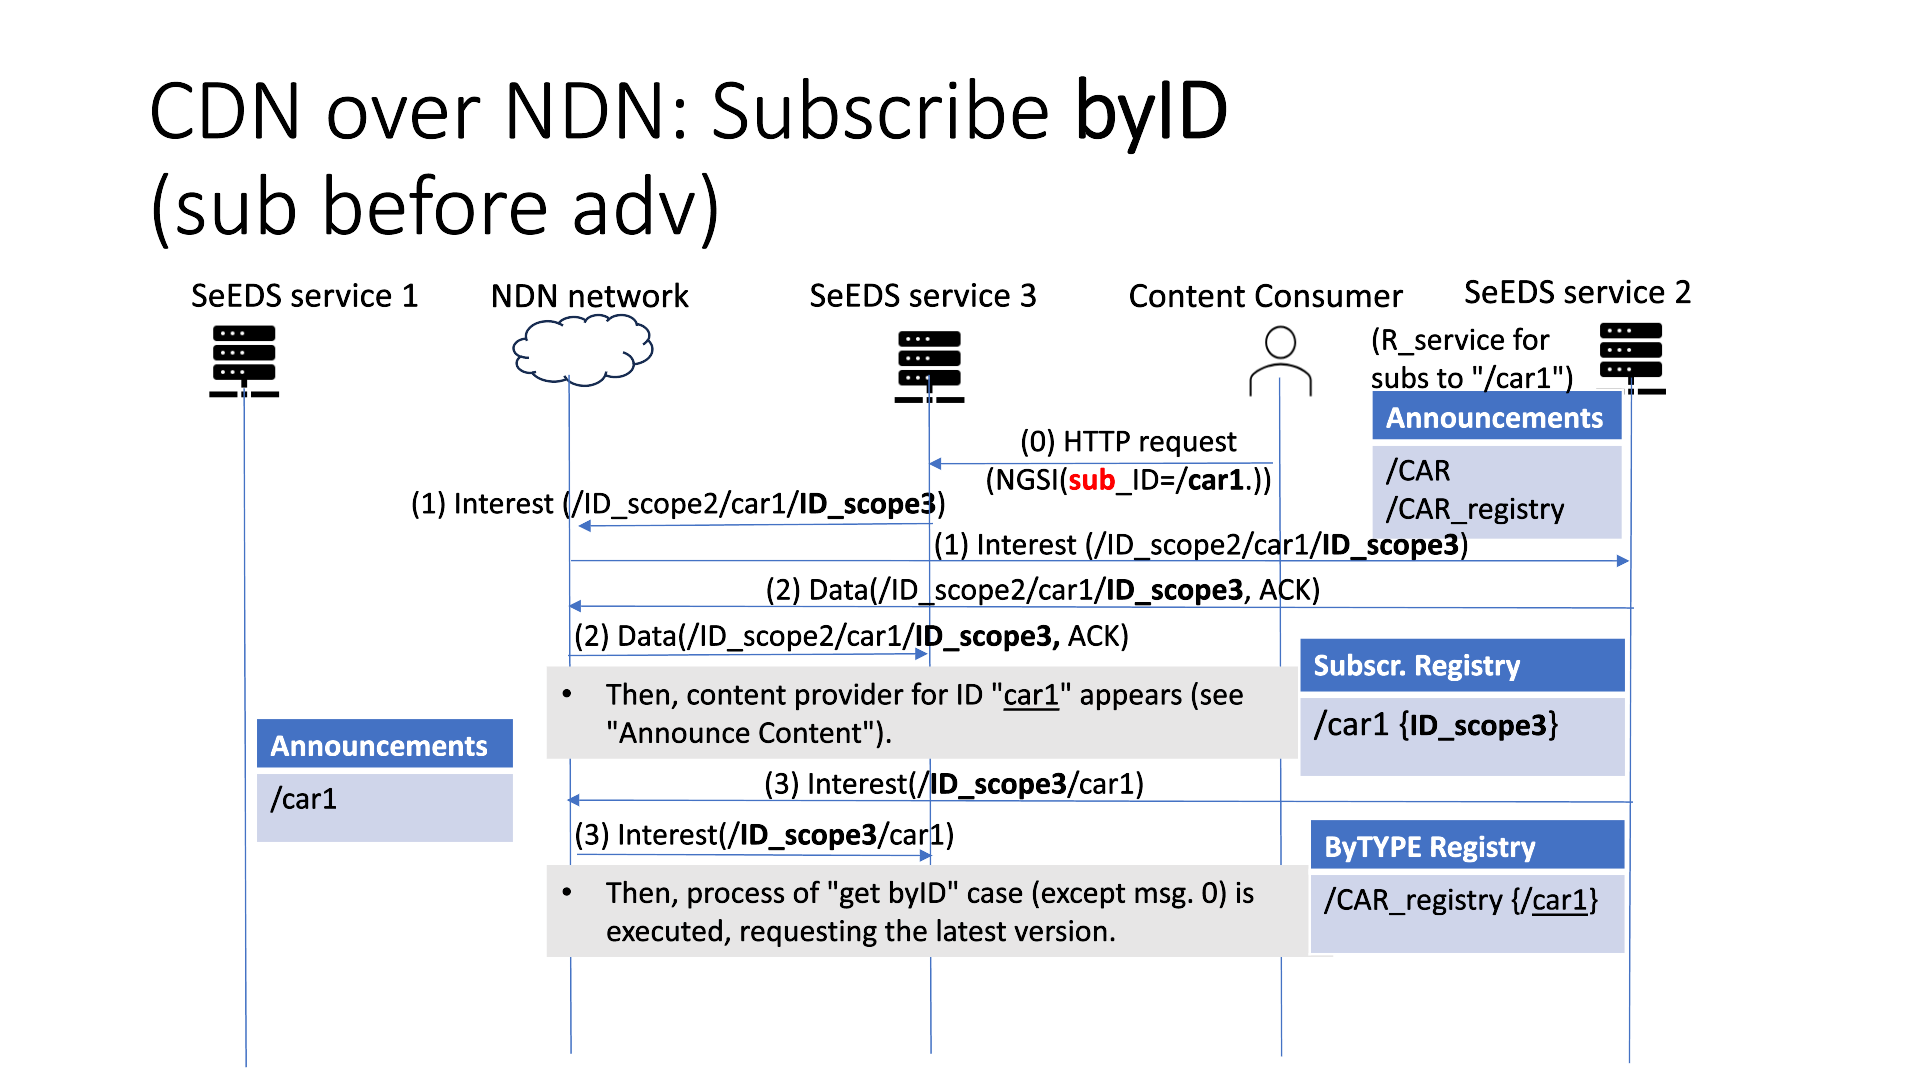
\includegraphics[width=0.8\linewidth]{images/subscribe_by_id.png}
    \caption{Subscribe by ID.}
    \label{fig:subscribe_by_id}
\end{figure}

\subsection{SUBSCRIPTIONS by TYPE}

Consumers can also subscribe to a specific \textit{@type}. In this case ( unlike \hyperref[subscriptions_by_id_section]{SUBSCRIBE by ID} ) , the subscription is linked to an already announced registry scope, so there is no need to compute a hash for the \textit{@type}. When the registry receives new data entries for that \textit{@type}, all subscribed consumers are notified that an update has occurred. 

As shown in message~\emph{(0)}, the consumer specifies the target \textit{@type} in the \emph{HTTP Request} sent to the SeEDS Service. Upon receiving the \emph{HTTP request}, the SeEDS Service expresses an \emph{Interest} toward the corresponding registry scope associated with that \textit{@type}, as illustrated in message~\emph{(1)}. The registry records the SeEDS Service that issued the Interest as a subscriber ( the diagram doesn't use \emph{ID\_SCOPE} but \emph{SeEDS\_ID} which is equivalent ) and replies with an \emph{ACK}, confirming that the subscription has been successfully registered, as shown in message~\emph{(2)}.

When new data is added to the registry for the subscribed \textit{@type}, the system notifies all registered subscribers, as depicted in message~\emph{(3)}. Upon receiving the notification, the SeEDS Service proceeds to perform a \hyperref[get_by_type_section]{GET by TYPE} operation to retrieve the updated content.


\begin{figure}[H]
    \centering
    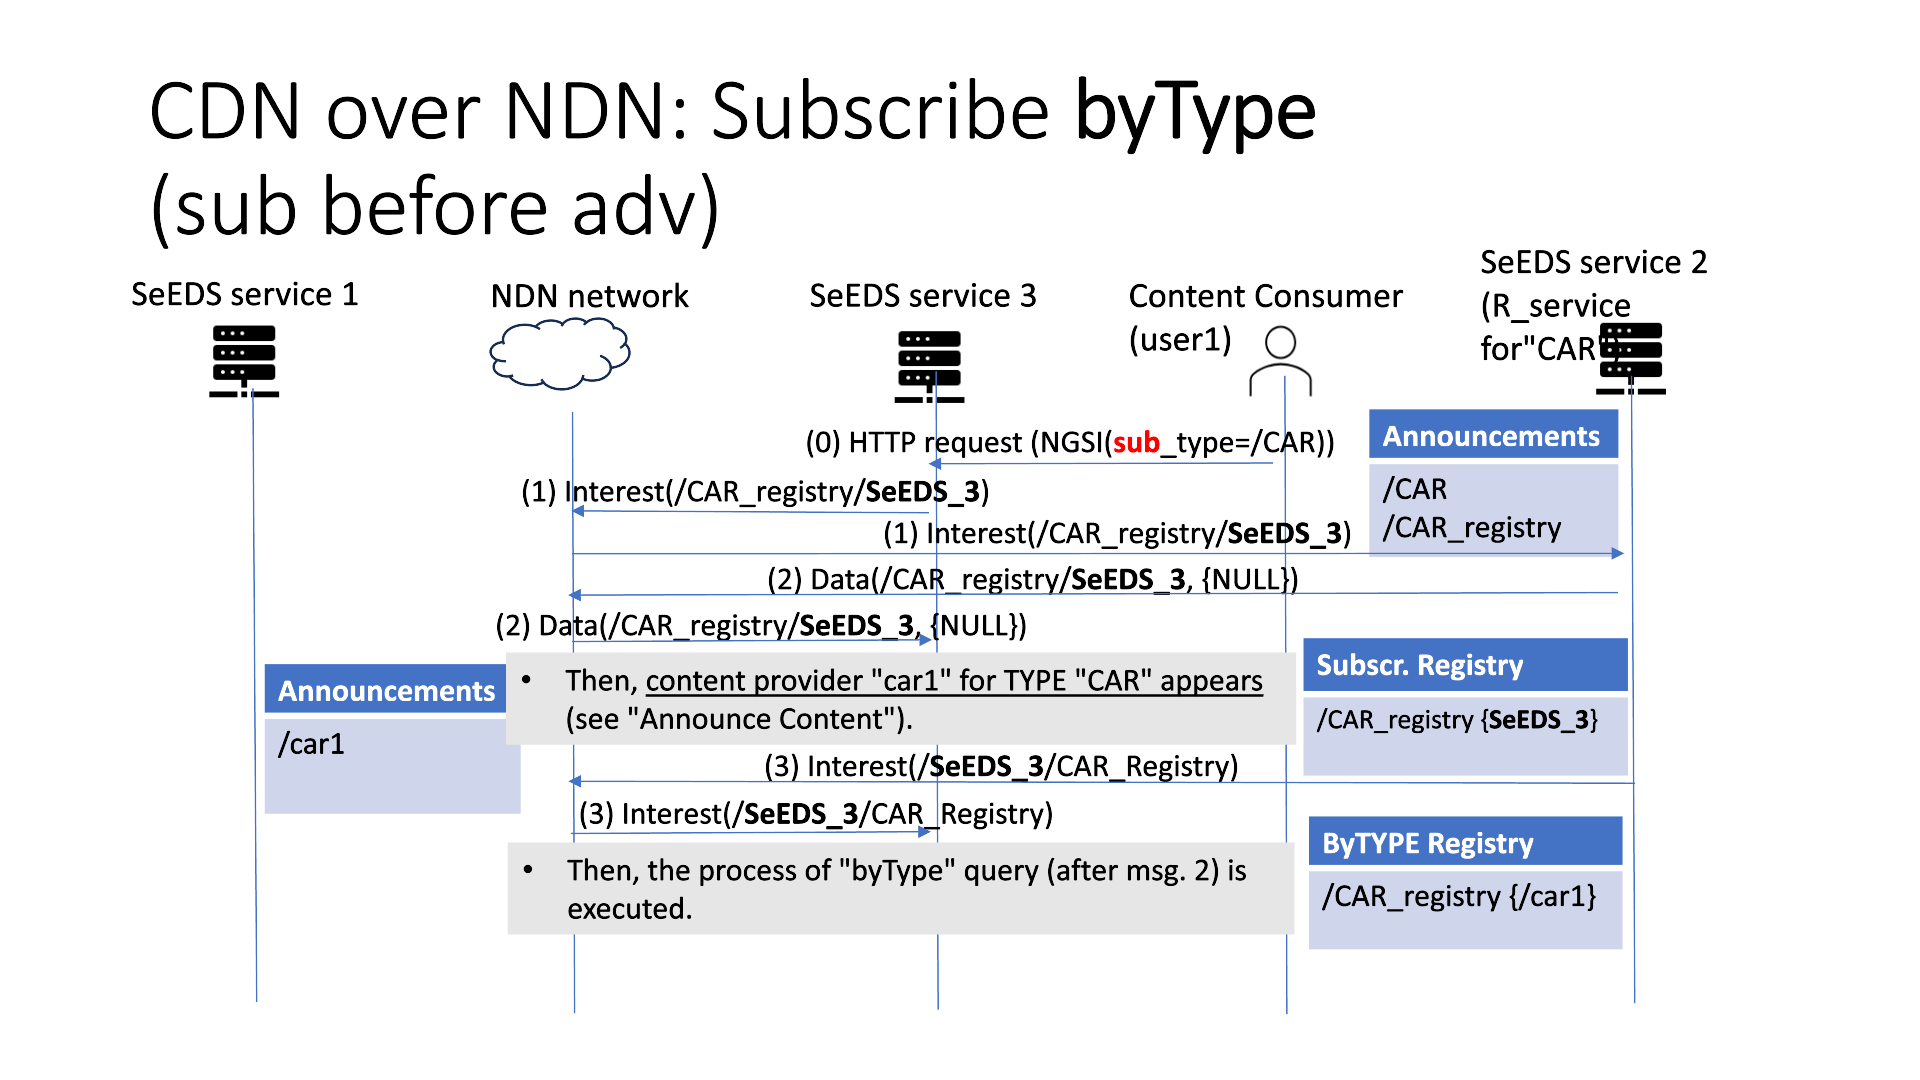
\includegraphics[width=0.8\linewidth]{images/subscribe_by_type.png}
    \caption{Subscribe by type.}
    \label{fig:subscribe_by_type}
\end{figure}

\pagebreak 

\subsection{Resilience}

Figure~\ref{fig:resilience} illustrates the message exchange that keeps a \emph{Secondary} SeEDS service converged with a remote \emph{Primary} over the NDN network. The \emph{Secondary} (left lane) runs two lightweight polling loops in parallel: (i) a \emph{state convergence} loop that tracks the \textit{state} of the Primary’s canonical store, and (ii) a \emph{liveness} loop that verifies that the remote service is responsive. Both loops use standardized Interests and Data packets and carry only minimal material (hashes, patches-snapshots, nonces) to limit overhead.

As shown in message~\emph{(0)}, the Primary has announced its state namespace \texttt{\{state\_2\}} in the NDN network, so other Services in the network can \emph{express interests} for it. The currently manually set Secondary initiates its state convergence loop by expressing an \emph{Interest} for the corresponding state hash, as depicted in message~\emph{(2)}. The returned \emph{Data} packet, shown in message~\emph{(3)}, contains the current hash and either a patch encoded as an RFC~6902 JSON Patch or an RFC~6902 Snapshot. The Secondary compares this hash with the locally stored version, and when a mismatch is detected, it applies the received patch or the snapshot, if the patch cannot be applied, to synchronize its local mirror with the Primary. 

Parallel to the state convergence loop, the Secondary executes a liveness verification loop to confirm that the Primary remains reachable. As illustrated in message~\emph{(1)}, the Primary advertises its liveness namespace \texttt{\{is\_alive\_2\}}. The Secondary periodically expresses \emph{Interest} packets containing a fresh nonce, as shown in message~\emph{(4)}. The Primary responds with a corresponding \emph{Data} packet that echoes the nonce and includes an acknowledgment, as depicted in message~\emph{(5)}. 

If the Secondary records consecutive failures in its liveness probes beyond a predefined threshold, it promotes itself to the \emph{Primary} and terminates the polling loop. This promotion is internally communicated to the SeEDS services through IPC, ensuring that operation continues uninterrupted even in the absence of the original Primary. This mechanism, SeEDS achieves distributed fault tolerance, maintaining service availability despite network or node failures.

\begin{figure}[H]
    \centering
    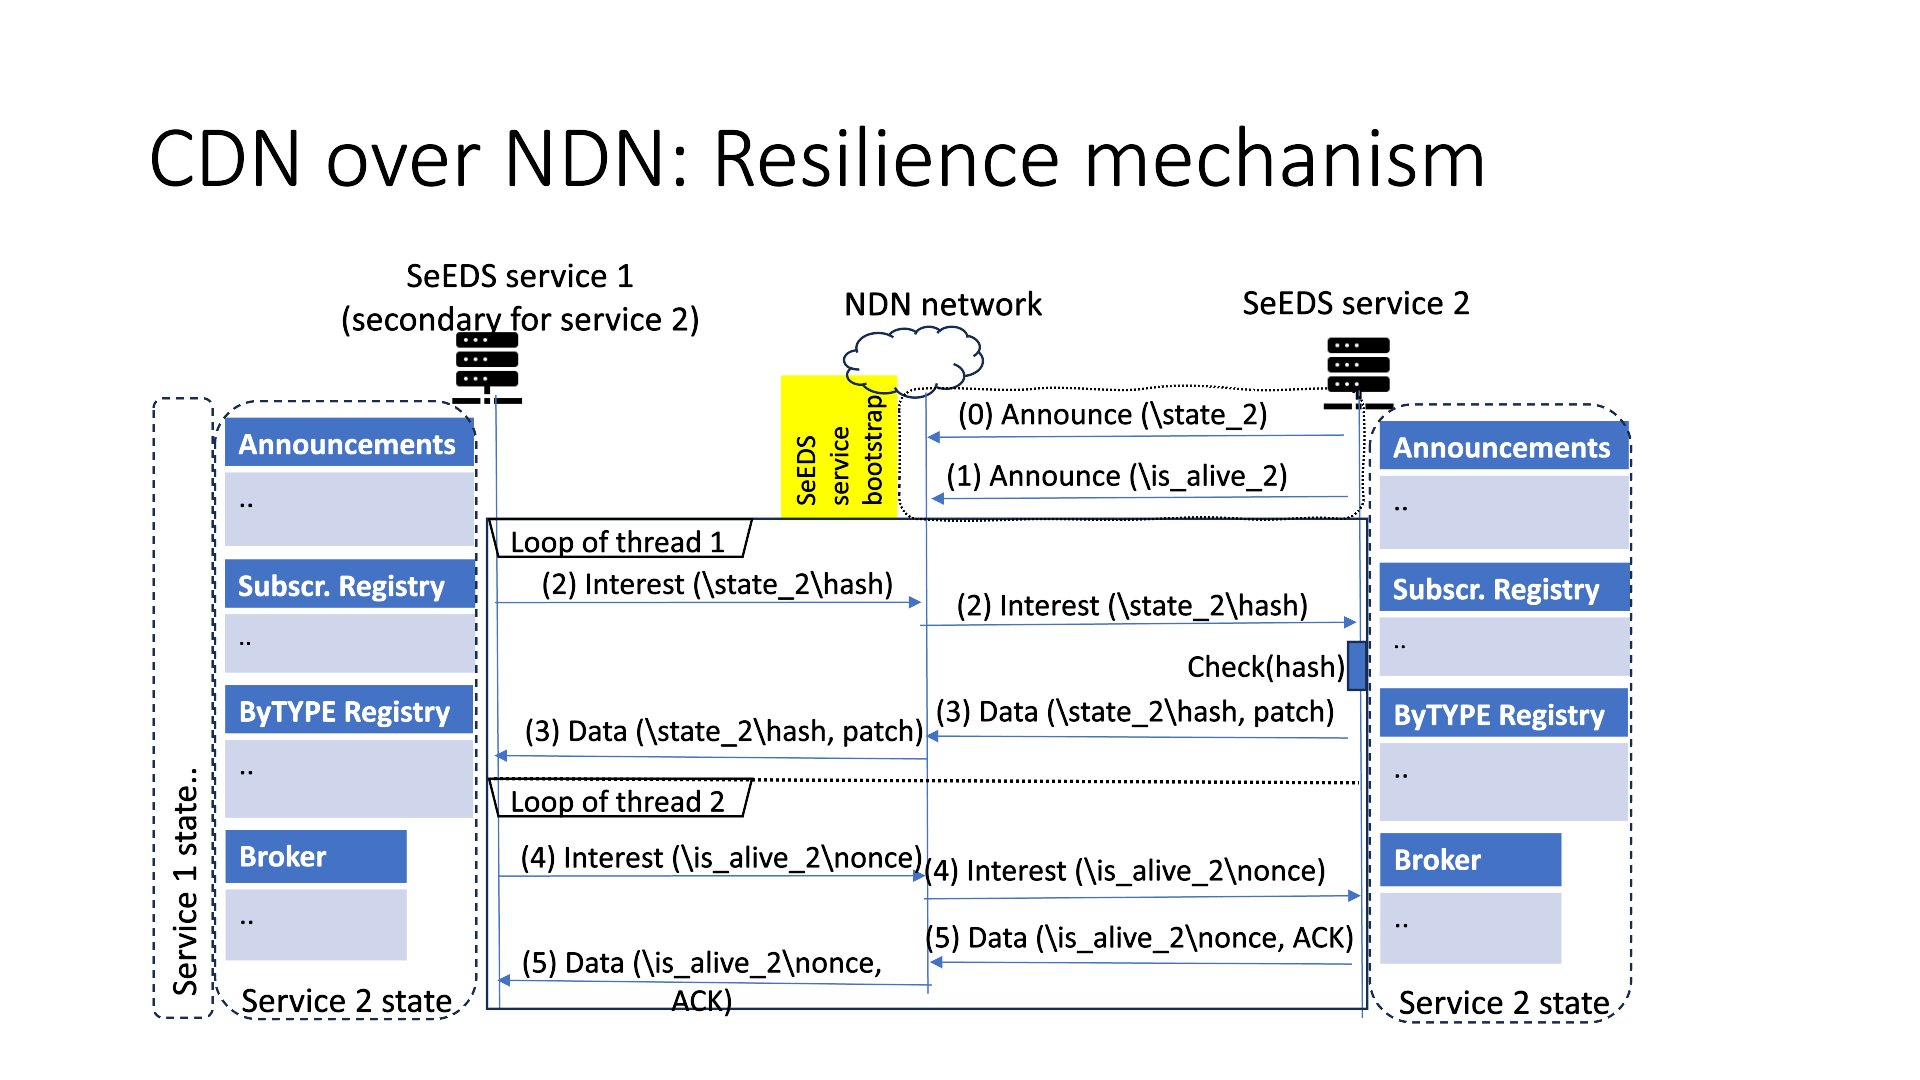
\includegraphics[width=0.8\linewidth]{images/resilience.png}
    \caption{Resilience message exchange in SeEDS.}
    \label{fig:resilience}
\end{figure}

\section{Experiments and KPIs}

\subsection{MiniNDN evalution}

Mini-NDN is a lightweight emulation framework designed to facilitate experimentation with Named Data Networking (NDN) in a controlled, reproducible environment. It is built on top of \textit{Mininet}, a popular network emulator that allows users to create virtual network topologies composed of multiple nodes, links, and switches within a single physical or virtual machine. Mini-NDN extends this capability by integrating the NDN Forwarding Daemon (NFD) and NDN tools into each emulated node, effectively transforming the Mininet network into a fully functional NDN deployment.

Each Mini-NDN node runs its own instance of NFD and can host NDN applications, such as producers and consumers, enabling realistic Interest/Data exchange over emulated network topologies. Mini-NDN supports custom configurations through topology and configuration files, making it straightforward to define arbitrary network graphs and specify per-node parameters such as faces, prefixes, and routing protocols.

Mini-NDN was employed to test and validate the functionality of the SeEDS prototype prior to its deployment in the global NDN testbed, ensuring correct operation before deployment to the actual testbed. Below, for brevity's sake, we are going to present the basic \emph{GET by ID} and \emph{GET by TYPE} requests. Everything else has been tested to ensure its correct operation and can be found on the \href{https://github.com/mmlab-aueb/SeEDS/blob/main/README.md}{official github repository}( \textbf{KPI 9} ).


\subsubsection{Topology}

The Mini-NDN emulation was deployed using a simple four-node topology defined in the configuration file shown in Listing~\ref{lst:minindn_conf}. The nodes are labeled \texttt{a}, \texttt{b}, \texttt{c}, and \texttt{d}, each running its own instance of the NDN Forwarding Daemon (NFD) with the log level set to \texttt{DEBUG}.

The connectivity between nodes is symmetric, with bidirectional links defined for each pair. Nodes \texttt{a}, \texttt{b}, and \texttt{c} form a triangular core interconnected with a delay of \texttt{10\,ms} per link, ensuring low-latency communication suitable for multi-hop experiments. Node \texttt{d} connects only to node \texttt{a}, also with a \texttt{10\,ms} delay, representing an edge node that communicates with the core through a single gateway.

\begin{figure}[H]
\centering
\begin{tikzpicture}[
    node/.style={circle, draw, thick, minimum size=9mm, font=\sffamily\bfseries},
    link/.style={-{Stealth[length=2mm]}-{Stealth[length=2mm]}, thick},
    >=Stealth
]
% Nodes
\node[node] (a) at (0,0) {a};
\node[node] (b) at (4,0) {b};
\node[node] (c) at (2,3) {c};
\node[node] (d) at (-2,0) {d};

% Core triangle links (bidirectional, 10 ms)
\draw[link] (a) -- node[above left,pos=0.5]{\small 10\,ms} (c);
\draw[link] (b) -- node[above right,pos=0.5]{\small 10\,ms} (c);
\draw[link] (a) -- node[below,pos=0.5]{\small 10\,ms} (b);

% Edge link for d (to a only)
\draw[link] (d) -- node[below,pos=0.5]{\small 10\,ms} (a);


\end{tikzpicture}
\caption{Mini-NDN topology: triangular core (a–b–c) with 10\,ms links; edge node d connected to a.}
\label{fig:minindn_topology}
\end{figure}

\begin{lstlisting}[language=minindnconf,caption={Mini-NDN topology .conf file},label={lst:minindn_conf}]
[nodes]
a: _ nfd-log-level=DEBUG
b: _ nfd-log-level=DEBUG
c: _ nfd-log-level=DEBUG
d: _ nfd-log-level=DEBUG

[links]
a:b delay=10ms
b:a delay=10ms
b:c delay=10ms
c:b delay=10ms
c:a delay=10ms
a:c delay=10ms
d:a delay=10ms
a:d delay=10ms
\end{lstlisting}


\pagebreak 

\subsubsection{GET by ID}

We have already published the \textit{@ids=car1,car2,car3} in the NDN network, through \emph{node A ( producer )}.


Let's try to retrieve the \textit{@id=car1} through \emph{node B}:

\begin{lstlisting}[language=log, caption={Node's B log after performing a GET by ID for car1}, label={lst:node-b-log-file-car1}]
[2025-09-25 00:33:40.583] [debug] [Consumer] Extracted content from message: /SNDS/car1/getByID:car1
[2025-09-25 00:33:40.583] [debug] [Consumer] Extracted content length from message: 23
[2025-09-25 00:33:40.583] [debug] [Consumer] Extracted message type from message: GET_BY_ID_REQUEST
[2025-09-25 00:33:40.583] [debug] [Consumer] Query.type: 
[2025-09-25 00:33:40.583] [debug] [Consumer] Query.id: car1
[2025-09-25 00:33:40.583] [info] [Consumer] Created name /SNDS/car1/temporalQuery:id%3Dcar1&type%3D&date%3D&count%3D&timeframe%3D&filters%3D
[2025-09-25 00:33:40.583] [info] [Consumer] Sending actual Interest /SNDS/car1/temporalQuery%3Aid%3Dcar1%26type%3D%26date%3D%26count%3D%26timeframe%3D%26filters%3D?CanBePrefix&Lifetime=6000
[2025-09-25 00:33:40.585] [info] [Consumer] Received Data with name: /SNDS/car1/temporalQuery%3Aid%3Dcar1%26type%3D%26date%3D%26count%3D%26timeframe%3D%26filters%3D in function onData
[2025-09-25 00:33:40.585] [info] [Consumer] Data packet payload: [
  {
    "": {
      "_id": "car1",
      "id": "car1",
      "timestamp": {
        "$date": 1758749528574
      },
      "type": "GENERIC"
    }
  }
] in function onData
[2025-09-25 00:33:40.585] [info] [Consumer] Parsed interest: Prefix: SNDS, Name: car1, Command: temporalQuery, Params: [id=car1, type=, date=, count=, timeframe=, filters=] in onData
[2025-09-25 00:33:40.585] [info] [Consumer] Temporal Query Reponse... 
\end{lstlisting}

\pagebreak 

Let's try to retrieve the \textit{@id=car2} through \emph{node C}:
\begin{lstlisting}[language=log, caption={Node's C log after performing a GET by ID for car2}, label={lst:node-c-log-file-car2}]
[2025-09-25 00:42:10.775] [debug] [Consumer] Extracted content from message: /SNDS/car2/getByID:car2
[2025-09-25 00:42:10.775] [debug] [Consumer] Extracted content length from message: 23
[2025-09-25 00:42:10.775] [debug] [Consumer] Extracted message type from message: GET_BY_ID_REQUEST
[2025-09-25 00:42:10.775] [debug] [Consumer] Query.type: 
[2025-09-25 00:42:10.775] [debug] [Consumer] Query.id: car2
[2025-09-25 00:42:10.775] [info] [Consumer] Created name /SNDS/car2/temporalQuery:id%3Dcar2&type%3D&date%3D&count%3D&timeframe%3D&filters%3D
[2025-09-25 00:42:10.775] [info] [Consumer] Sending actual Interest /SNDS/car2/temporalQuery%3Aid%3Dcar2%26type%3D%26date%3D%26count%3D%26timeframe%3D%26filters%3D?CanBePrefix&Lifetime=6000
[2025-09-25 00:42:10.777] [info] [Consumer] Received Data with name: /SNDS/car2/temporalQuery%3Aid%3Dcar2%26type%3D%26date%3D%26count%3D%26timeframe%3D%26filters%3D in function onData
[2025-09-25 00:42:10.777] [info] [Consumer] Data packet payload: [
  {
    "": {
      "_id": "car2",
      "id": "car2",
      "timestamp": {
        "$date": 1758749532578
      },
      "type": "GENERIC"
    }
  }
] in function onData
[2025-09-25 00:42:10.777] [info] [Consumer] Parsed interest: Prefix: SNDS, Name: car2, Command: temporalQuery, Params: [id=car2, type=, date=, count=, timeframe=, filters=] in onData
\end{lstlisting}

\pagebreak

Let's try to retrieve the \textit{@id=car3} through \emph{node D}:
\begin{lstlisting}[language=log, caption={Node's D log after performing a GET by ID for car3}, label={lst:node-d-log-file-car3}]
[2025-09-25 00:38:19.399] [debug] [Consumer] Extracted content from message: /SNDS/car3/getByID:car3
[2025-09-25 00:38:19.399] [debug] [Consumer] Extracted content length from message: 23
[2025-09-25 00:38:19.399] [debug] [Consumer] Extracted message type from message: GET_BY_ID_REQUEST
[2025-09-25 00:38:19.399] [debug] [Consumer] Query.type: 
[2025-09-25 00:38:19.399] [debug] [Consumer] Query.id: car3
[2025-09-25 00:38:19.399] [info] [Consumer] Created name /SNDS/car3/temporalQuery:id%3Dcar3&type%3D&date%3D&count%3D&timeframe%3D&filters%3D
[2025-09-25 00:38:19.399] [info] [Consumer] Sending actual Interest /SNDS/car3/temporalQuery%3Aid%3Dcar3%26type%3D%26date%3D%26count%3D%26timeframe%3D%26filters%3D?CanBePrefix&Lifetime=6000
[2025-09-25 00:38:19.400] [info] [Consumer] Received Data with name: /SNDS/car3/temporalQuery%3Aid%3Dcar3%26type%3D%26date%3D%26count%3D%26timeframe%3D%26filters%3D in function onData
[2025-09-25 00:38:19.400] [info] [Consumer] Data packet payload: [
  {
    "": {
      "_id": "car3",
      "id": "car3",
      "timestamp": {
        "$date": 1758749534580
      },
      "type": "GENERIC"
    }
  }
] in function onData
[2025-09-25 00:38:19.400] [info] [Consumer] Parsed interest: Prefix: SNDS, Name: car3, Command: temporalQuery, Params: [id=car3, type=, date=, count=, timeframe=, filters=] in onData
\end{lstlisting}

\pagebreak

Here are the logs of the Producer, receiving requests from the other Nodes that requested the \textit{@id}: 

\begin{lstlisting}[language=log, caption={Producer Log File},label={lst:producer-log-file}]
[2025-09-25 00:33:40.583] [info] [Producer] Received interest in function: onInterest, name: /SNDS/car1/temporalQuery%3Aid%3Dcar1%26type%3D%26date%3D%26count%3D%26timeframe%3D%26filters%3D
[2025-09-25 00:33:40.583] [info] [Producer] Parsed interest: Prefix: SNDS, Name: car1, Command: temporalQuery, Params: [id=car1, type=, date=, count=, timeframe=, filters=]
[2025-09-25 00:33:40.583] [debug] [Producer] Created interest response: /SNDS/car1/temporalQuery%3Aid%3Dcar1%26type%3D%26date%3D%26count%3D%26timeframe%3D%26filters%3D in: process_temporal_query_interest
[2025-09-25 00:33:40.583] [debug] [Producer] TemporalQuery → id: car1, date: , type: , timeframe: , count: , filters: 
[2025-09-25 00:33:40.583] [debug] [Producer] Requesting to endpoint: /temporal-query?id=car1&type=&count=&date=&timeframe=&filters=
[2025-09-25 00:33:40.585] [info] [Producer] Successfully queried /temporal-query
[2025-09-25 00:33:40.585] [debug] [Producer] Sending data to the NDN…
[2025-09-25 00:35:26.584] [info] [Producer] Received interest in function: onInterest, name: /SNDS/SNDS_ID_scope_0/scopeNotification%3Acar2%26%26SNDS_ID_scope_2
[2025-09-25 00:35:26.584] [info] [Producer] Parsed interest: Prefix: SNDS, Name: SNDS_ID_scope_0, Command: scopeNotification, Params: [car2, , SNDS_ID_scope_2]
[2025-09-25 00:35:26.584] [info] [Producer] [BY_ID] Subscription notification for ID name car2 and/or TYPE: .
[2025-09-25 00:35:26.584] [info] [Producer] No subscribers found for ID: car2 and/or TYPE: .
[2025-09-25 00:35:26.584] [info] [Producer] Responding to interest: /SNDS/SNDS_ID_scope_0/scopeNotification%3Acar2%26%26SNDS_ID_scope_2
[2025-09-25 00:35:26.584] [debug] [Producer] Sending data to the NDN…
[2025-09-25 00:35:41.239] [info] [Producer] Received interest in function: onInterest, name: /SNDS/car3/temporalQuery%3Aid%3Dcar3%26type%3D%26date%3D%26count%3D%26timeframe%3D%26filters%3D
[2025-09-25 00:35:41.239] [info] [Producer] Parsed interest: Prefix: SNDS, Name: car3, Command: temporalQuery, Params: [id=car3, type=, date=, count=, timeframe=, filters=]
[2025-09-25 00:35:41.239] [debug] [Producer] Created interest response: /SNDS/car3/temporalQuery%3Aid%3Dcar3%26type%3D%26date%3D%26count%3D%26timeframe%3D%26filters%3D in: process_temporal_query_interest
[2025-09-25 00:35:41.239] [debug] [Producer] TemporalQuery → id: car3, date: , type: , timeframe: , count: , filters: 
[2025-09-25 00:35:41.239] [debug] [Producer] Requesting to endpoint: /temporal-query?id=car3&type=&count=&date=&timeframe=&filters=
[2025-09-25 00:35:41.241] [info] [Producer] Successfully queried /temporal-query
[2025-09-25 00:35:41.241] [debug] [Producer] Sending data to the NDN… 
\end{lstlisting}

We can see that within the described Mini-NDN topology, node \texttt{a} acts as the producer responsible for serving data associated with specific \textit{@ids}. Because all nodes are interconnected, any node in the network can retrieve content produced by node \texttt{a}. Nodes \texttt{b} and \texttt{c} communicate with \texttt{a} via direct paths within the triangular core, enabling efficient Interest forwarding and Data return. Node \texttt{d}, which is connected only to \texttt{a}, retrieves data through its single 10\,ms link without possibly requiring any intermediate forwarding. This configuration ensures that every node in the network has a reachable route to the producer, allowing all consumers to successfully issue Interests and receive corresponding Data packets for a given \textit{@id}, thus validating correct NDN forwarding and content retrieval in the SeEDS prototype.


\subsubsection{GET by TYPE}

\subsection{Resilience (KPI 8)}
\subsection{NDN-testbed (KPI 6)}
\section{Conclusion}

\end{document}
